\chapter{Proposed Solution}
\label{chap:ProposedSolution}

This chapter contains a detailed description of the final solution: data preparation, approaches taken to implement the n-gram sorters, and various engineering details.

\section{Solution Overview}
\label{sec:ProposedSolution-Overview}
The objective of this implementation is the following: suggest the most likely tokens at every step of the completion process. The main idea is to leave the existing, AST-based code completion engine in place, and just enhance the sorting strategy. For this, I implemented two separate sorters based on n-gram models. That means that after the list of completion candidates is proposed, it gets sorted based on each n-gram's probability, so that the most relevant completions are shown first.

\subsection{Unigram Sorting}
The first implementation, unigram-based sorting, is based on the 1-gram analysis, which means that we only take into consideration the actual token being completed. The implementation of the unigram model itself comes down to calculating individual token frequencies, i.e. the number of occurrences of each token in the source code. Then the completion candidates are sorted according to each one's frequency. In Figures \ref{fig:unigramCode1}, \ref{fig:unigramCode2} and \ref{fig:unigramCode3} you can see the frequencies data being passed to the sorter, and then the completions being sorted based on that information:

\begin{figure}[H]
    \centering
    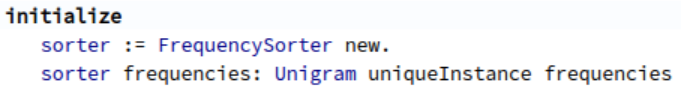
\includegraphics[width=0.9\linewidth]{images/unigramCode1.png}
    \caption{The unigram sorter implementation: passing the frequencies to the sorter}
    \label{fig:unigramCode1}
\end{figure}

\begin{figure}[H]
    \centering
    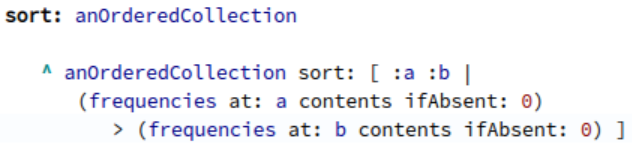
\includegraphics[width=0.9\linewidth]{images/unigramCode3.png}
    \caption{The sorter implementation: sorting the candidates according to their frequencies}
    \label{fig:unigramCode2}
\end{figure}

\begin{figure}[H]
    \centering
    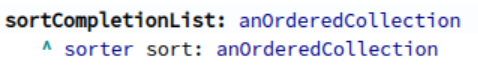
\includegraphics[width=0.9\linewidth]{images/unigramCode2.png}
    \caption{The unigram sorter implementation: returning the results sorted in the code above}
    \label{fig:unigramCode3}
\end{figure}

\subsection{Bigram Sorting}
The second, more advanced implementation, is the bigram sorting strategy. As an n-gram model where \textit{n=2}, it relies on both the token currently being completed and the history -- in this case, one token before the current one. I then get the previous token from the part of code where the completion is being called. After that, once the history word and each completion candidate are assembled together into respective pairs of tokens, I calculate the probability of each of the ngram sequences. Then the joint sequence probabilities are used for sorting each completion candidate (second word of the sequence). Figure \ref{fig:bigramCode} shows how the sorting method looks in the end:

\begin{figure}[H]
    \centering
    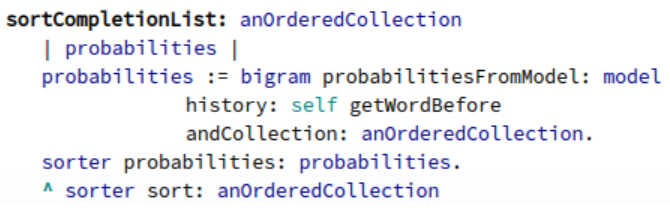
\includegraphics[width=0.9\linewidth]{images/bigramCode.png}
    \caption{The bigram sorter implementation: receives the list of completions, gets the word before from context, trains the model, and sorts the completions based on sequence probabilities}
    \label{fig:bigramCode}
\end{figure}

\section{Implementation Details}
\label{sec:ProposedSolution-Implementation}
\subsection{Data Preparation}
Before implementing the sorting strategies, I needed to train the n-gram models. The first step was to get the dataset. For this I retrieved the Pharo source code which was collected by \cite{Zait20a} for their research on characterising Pharo code. The data came from 50 projects, which consisted of 824 packages, 13,935 classes, and 151,717 methods. In particular, I used the dataset where the source code was already split into tokens and respective token types for each method. Among the regular alphabetic tokens, the delimiters and non-alphabetic tokens were included as well. For example, a comment such as '"Here is a comment for this method"' or a delimiter '.' would be considered separate tokens, and their respective token types would be 'COM' and 'DOT'.

Due to a large number of tokens in the dataset, I needed to be mindful of potential time constraints, as the lookup of n-gram probabilities used for sorting had to be fast enough to not make the developer pause and wait for it. Throughout the course of the experiment, I came up with various ways to additionally reduce the dataset. Each of those attempts will be described in the following subsection.

\subsection{Engineering Details}
Before training our models, we took some data preparation steps, additionally cleaning the data, such as deleting some rows with token and token type mismatch, eliminating double tabs and replacing them with placeholders, and splitting token and token types into separate columns. After that, when recording token frequencies for the unigram model, we decided we would write the results to file, for faster lookup for the sorting. However, even with that approach, we faced a problem: as the initial number of tokens was around 150k, the lookup was slow enough to be noticeable and break the developer's flow when typing. 

Our approach to improve the time efficiency was to set a certain threshold for the number of occurences, and to cut off all the tokens with frequencies below it. We put the threshold equal to 10, meaning if the token occured less than 10 times throughout the whole history, it was irrelevant enough to be discarded. This way, we were able to cut off most of the miscellaneous, rarely encountered tokens, and shortened our dataset from 150k to just 16k entries. This made the frequencies lookup during completion sorting very fast and, as a result, it was now possible to type and use completion information without any delays.

For comparison, below are the results for the unigram sorter before the cut off (150k tokens; Fig. \ref{fig:sorterSlow}) and after (16k tokens; Fig. \ref{fig:sorterFast}).

\begin{figure}[H]
    \centering
    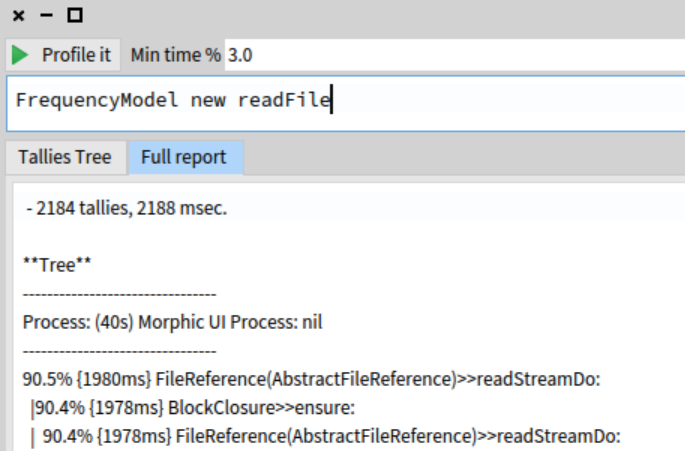
\includegraphics[width=0.9\linewidth]{images/sorterSlow.png}
    \caption{It takes 2k ms for completion to be called pre-cut off}
    \label{fig:sorterSlow}
\end{figure}

\begin{figure}[H]
    \centering
    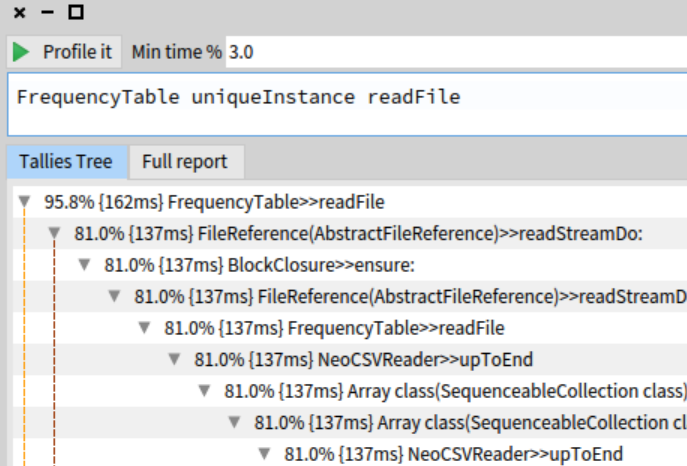
\includegraphics[width=0.9\linewidth]{images/sorterFast.png}
    \caption{It takes only 160 ms after cut off}
    \label{fig:sorterFast}
\end{figure}

The one-time tokens, such as custom strings and comments, were not as relevant to us during implementing the unigram sorting strategy, however when we moved on to implementing the bigram sorter, the bigram model became "too heavy" due to many combinations of such tokens, and needed to be additionally reduced. Our solution was to go back to the data processing step and replace those "one-time" tokens with placeholders. In particular, we added placeholders for strings, comments, symbols, characters, arrays and numbers (such as all strings being written as <str> and all numbers as <num>). This allowed us to greatly reduce both the number of total tokens and subsequent ngram sequences, which helped both the bigram and the unigram model, as well as the lookup speed.

\subsection{N-gram Library Extension}
The bigram model trained on source code data was implemented with the help of the NgramModel library \footnote{\url{https://github.com/pharo-ai/NgramModel}}. In the process of working on implementing the model, we extended the existing library with the following functionality:
\begin{itemize}
    \item functionality to filter the table of ngrams (cut off ngram sequences with counts below a certain threshold)
    \item adding writing to and reading ngram models from file
\end{itemize}

\section{Summary}
\label{sec:ProposedSolution-Summary}
The unigram-based sorter is available in the Pharo IDE as the FrequencyCompletionSorter, and the bigram-based as the BigramCompltionSorter -- i.e. they can already be used by enabling the respective sorting option in the Settings.

A short summary of the implementation, along with data preparation and engineering details:
\begin{itemize}
    \item the data used to train the models came from 50 projects implemented in Pharo; in the dataset the source code was already split into tokens and token types
    \item in the data, delimiters and non-alphabetic tokens, as well as comments, were all considered to be separate tokens
    \item for unigram sorting, individual token frequencies were extracted; the sorting of completion candidates was based on the number of occurences of each token by itself
    \item for bigram sorting, completion candidates were added to the previous token to form sequences of bigrams, whose probability was later calculated and recorded to file; the sorting was based on the sequence probability but it was only applied to individually displayed completion candidates
    \item both sorting strategies can be enabled to be used in the Pharo IDE
    \item different approaches were taken to reduce the sizes of models and speed up lookup and sorting time; among them: cleaning up tokens and sequences with occurences below a certain threshold, and replacing irrelevant "one-time" tokens (such as specific strings, numbers, characters, and so on) with general placeholders (such as <str>, <num>, etc.)
    \item in the process of working on the bigram sorting strategy, the NgramModel Pharo library that was used for this approach was addiitionally extended with new functionality
\end{itemize}

\begin{figure}[H]
    \centering
    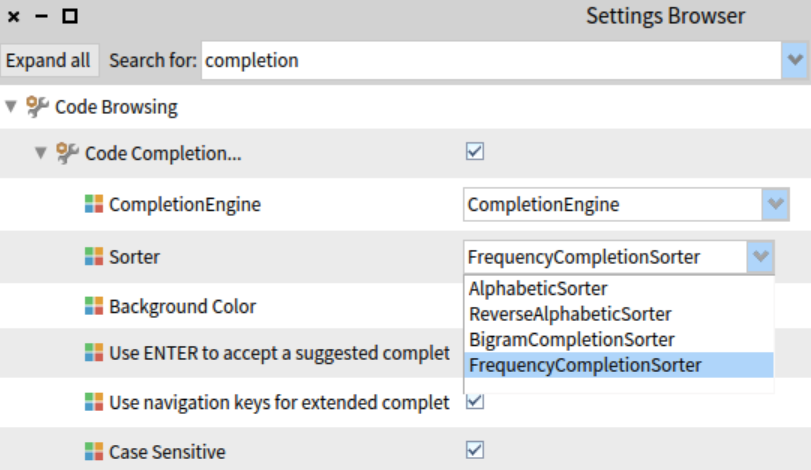
\includegraphics[width=0.9\linewidth]{images/settings.png}
    \caption{The Settings window in the Pharo IDE}
    \label{fig:settings}
\end{figure}